% ============================================================= %
%  Template LaTeX pour Quarto — Mémoire CNAM style
% ============================================================= 
\documentclass{article}

\usepackage{color}
\usepackage{fancyvrb}
\newcommand{\VerbBar}{|}
\newcommand{\VERB}{\Verb[commandchars=\\\{\}]}
\DefineVerbatimEnvironment{Highlighting}{Verbatim}{commandchars=\\\{\}}
% Add ',fontsize=\small' for more characters per line
\usepackage{framed}
\definecolor{shadecolor}{RGB}{241,243,245}
\newenvironment{Shaded}{\begin{snugshade}}{\end{snugshade}}
\newcommand{\AlertTok}[1]{\textcolor[rgb]{0.68,0.00,0.00}{#1}}
\newcommand{\AnnotationTok}[1]{\textcolor[rgb]{0.37,0.37,0.37}{#1}}
\newcommand{\AttributeTok}[1]{\textcolor[rgb]{0.40,0.45,0.13}{#1}}
\newcommand{\BaseNTok}[1]{\textcolor[rgb]{0.68,0.00,0.00}{#1}}
\newcommand{\BuiltInTok}[1]{\textcolor[rgb]{0.00,0.23,0.31}{#1}}
\newcommand{\CharTok}[1]{\textcolor[rgb]{0.13,0.47,0.30}{#1}}
\newcommand{\CommentTok}[1]{\textcolor[rgb]{0.37,0.37,0.37}{#1}}
\newcommand{\CommentVarTok}[1]{\textcolor[rgb]{0.37,0.37,0.37}{\textit{#1}}}
\newcommand{\ConstantTok}[1]{\textcolor[rgb]{0.56,0.35,0.01}{#1}}
\newcommand{\ControlFlowTok}[1]{\textcolor[rgb]{0.00,0.23,0.31}{\textbf{#1}}}
\newcommand{\DataTypeTok}[1]{\textcolor[rgb]{0.68,0.00,0.00}{#1}}
\newcommand{\DecValTok}[1]{\textcolor[rgb]{0.68,0.00,0.00}{#1}}
\newcommand{\DocumentationTok}[1]{\textcolor[rgb]{0.37,0.37,0.37}{\textit{#1}}}
\newcommand{\ErrorTok}[1]{\textcolor[rgb]{0.68,0.00,0.00}{#1}}
\newcommand{\ExtensionTok}[1]{\textcolor[rgb]{0.00,0.23,0.31}{#1}}
\newcommand{\FloatTok}[1]{\textcolor[rgb]{0.68,0.00,0.00}{#1}}
\newcommand{\FunctionTok}[1]{\textcolor[rgb]{0.28,0.35,0.67}{#1}}
\newcommand{\ImportTok}[1]{\textcolor[rgb]{0.00,0.46,0.62}{#1}}
\newcommand{\InformationTok}[1]{\textcolor[rgb]{0.37,0.37,0.37}{#1}}
\newcommand{\KeywordTok}[1]{\textcolor[rgb]{0.00,0.23,0.31}{\textbf{#1}}}
\newcommand{\NormalTok}[1]{\textcolor[rgb]{0.00,0.23,0.31}{#1}}
\newcommand{\OperatorTok}[1]{\textcolor[rgb]{0.37,0.37,0.37}{#1}}
\newcommand{\OtherTok}[1]{\textcolor[rgb]{0.00,0.23,0.31}{#1}}
\newcommand{\PreprocessorTok}[1]{\textcolor[rgb]{0.68,0.00,0.00}{#1}}
\newcommand{\RegionMarkerTok}[1]{\textcolor[rgb]{0.00,0.23,0.31}{#1}}
\newcommand{\SpecialCharTok}[1]{\textcolor[rgb]{0.37,0.37,0.37}{#1}}
\newcommand{\SpecialStringTok}[1]{\textcolor[rgb]{0.13,0.47,0.30}{#1}}
\newcommand{\StringTok}[1]{\textcolor[rgb]{0.13,0.47,0.30}{#1}}
\newcommand{\VariableTok}[1]{\textcolor[rgb]{0.07,0.07,0.07}{#1}}
\newcommand{\VerbatimStringTok}[1]{\textcolor[rgb]{0.13,0.47,0.30}{#1}}
\newcommand{\WarningTok}[1]{\textcolor[rgb]{0.37,0.37,0.37}{\textit{#1}}}

% ── Packages essentiels ─────────────────────────────────────── 
\usepackage{geometry}
\geometry{a4paper, top=2.5cm, bottom=2.5cm, left=3cm, right=3cm}

\usepackage{microtype}
\usepackage{lmodern}

% ── Couleurs ───────────────────────────────────────────────── 
\usepackage{xcolor}
\usepackage{colortbl}
\definecolor{cnamred}{RGB}{210, 35, 42}
\definecolor{cnamgray}{RGB}{90, 90, 90}
\definecolor{sectionblue}{RGB}{31, 73, 125}
\definecolor{lightgray}{RGB}{245, 245, 245}
\definecolor{rulegray}{RGB}{180, 180, 180}
\definecolor{shadecolor}{RGB}{248, 248, 248}

% ── Graphiques & mise en page ──────────────────────────────── 
\usepackage{graphicx}

% ── Fix pour les images Quarto (pandocbounded) ─────────────── 
\makeatletter
\def\maxwidth{\ifdim\Gin@nat@width>\linewidth\linewidth\else\Gin@nat@width\fi}
\def\maxheight{\ifdim\Gin@nat@height>\textheight\textheight\else\Gin@nat@height\fi}

\newsavebox\pandoc@box
\newcommand*\pandocbounded[1]{%
  \sbox\pandoc@box{#1}%
  \Gscale@div\@tempa{\textheight}{\dimexpr\ht\pandoc@box+\dp\pandoc@box\relax}%
  \Gscale@div\@tempb{\linewidth}{\wd\pandoc@box}%
  \ifdim\@tempb\p@<\@tempa\p@\let\@tempa\@tempb\fi%
  \ifdim\@tempa\p@<\p@\scalebox{\@tempa}{\usebox\pandoc@box}%
  \else\usebox{\pandoc@box}%
  \fi%
}
\makeatother

\usepackage{tikz}
\usepackage{calc}
\usepackage{tabularx}
\usepackage{booktabs}
\usepackage{array}
\usepackage{multirow}
\usepackage{ragged2e}

% ── Typographie des titres ─────────────────────────────────── 
\usepackage{titlesec}

\titleformat{\section}
  {\color{sectionblue}\large\bfseries}
  {\thesection.}{0.6em}{}
  [{\color{rulegray}\vspace{2pt}{\titlerule[0.4pt]}\vspace{4pt}}]

\titleformat{\subsection}
  {\color{sectionblue}\normalsize\bfseries}
  {\thesubsection}{0.6em}{}

\titleformat{\subsubsection}
  {\color{cnamgray}\normalsize\itshape\bfseries}
  {\thesubsubsection}{0.6em}{}

\titlespacing*{\section}{0pt}{18pt}{8pt}
\titlespacing*{\subsection}{0pt}{14pt}{5pt}
\titlespacing*{\subsubsection}{0pt}{10pt}{4pt}

% ── Table des matières ─────────────────────────────────────── 
\usepackage{tocloft}
\renewcommand{\cftsecfont}{\bfseries\color{sectionblue}}
\renewcommand{\cftsecpagefont}{\bfseries\color{sectionblue}}
\renewcommand{\cftsubsecfont}{\color{cnamgray}}
\renewcommand{\cftsubsecpagefont}{\color{cnamgray}}
\renewcommand{\cftsecleader}{\cftdotfill{\cftdotsep}}
\setlength{\cftbeforesecskip}{4pt}

% ── Hyperliens ─────────────────────────────────────────────── 
\usepackage{hyperref}
\hypersetup{
  colorlinks=true,
  linkcolor=sectionblue,
  urlcolor=cnamred,
  citecolor=cnamgray,
  pdfborder={0 0 0}
}

% ── En-têtes et pieds de page ──────────────────────────────── 
\usepackage{fancyhdr}
\pagestyle{fancy}
\fancyhf{}
\fancyhead[L]{\small\color{cnamgray}\textit{Cluster analysis}}
\fancyhead[R]{\small\color{cnamgray}Arsène MBABEH - Raphaël PÉNÉ - Oscar JOSEPH--GENESLAY}
\fancyfoot[C]{\small\color{cnamgray}\thepage}
\renewcommand{\headrulewidth}{0.4pt}
\renewcommand{\footrulewidth}{0pt}

% ── Mathématiques ──────────────────────────────────────────── 
\usepackage{amsmath, amssymb, amsthm}

% ── Bibliographie ──────────────────────────────────────────── 

\usepackage[backend=biber, style=apa]{biblatex}
\addbibresource{references.bib}

% ── Utilitaires Pandoc / Quarto ────────────────────────────── 
\usepackage{longtable}
\usepackage{float}
\usepackage{caption}
\captionsetup{font=small, labelfont={bf,color=sectionblue}, textfont=it}
\usepackage{subcaption}
\usepackage{framed}
\usepackage{wrapfig}
\usepackage{pdflscape}
\usepackage{threeparttable}
\usepackage{threeparttablex}
\usepackage[normalem]{ulem}
\usepackage{makecell}

% ── Fix bug longtable : Pandoc génère \begin{longtable}[]{} ────
%    L'argument optionnel vide [] est interprété comme le compteur
%    "none" qui n'existe pas → on le crée silencieusement.
\makeatletter
\@ifundefined{c@none}{\newcounter{none}}{}
\makeatother

\providecommand{\tightlist}{%
  \setlength{\itemsep}{2pt}\setlength{\parskip}{0pt}}

% ── Interligne & paragraphes ───────────────────────────────── 
\usepackage{setspace}
\setstretch{1.15}
\setlength{\parskip}{6pt}
\setlength{\parindent}{0pt}


% ============================================================= %
%  DOCUMENT
% ============================================================= 
\begin{document}

% ── PAGE DE GARDE ──────────────────────────────────────────── 
\begin{titlepage}
\thispagestyle{empty}

\begin{tikzpicture}[remember picture, overlay]
  \node[anchor=north east, xshift=-1.5cm, yshift=-1.2cm]
    at (current page.north east) {%
      
\includegraphics[width=4cm, keepaspectratio]{logo_cnam.jpg}
    };
\end{tikzpicture}

\vspace*{2cm}

\begin{center}
  {\large\bfseries{Le Conservatoire National des Arts et M\'{e}tiers}}\\[0.4cm]
  \textcolor{rulegray}{\rule{10cm}{0.4pt}}\\[0.6cm]
  {\normalsize Rapport sur la reproductibilité d'un article scientifique sur le clustering}\\[0.4cm]
  {\normalsize\bfseries Fouille de donn\'{e}es}\\[0.5cm]
  {\small \textit{30 mai 2026} par}\\[0.5cm]
  {\normalsize\bfseries Arsène MBABEH - Raphaël PÉNÉ - Oscar JOSEPH--GENESLAY}\\[0.4cm]
  {\normalsize Promotion (2025-2026)}\\[0.5cm]
  \textcolor{rulegray}{\rule{10cm}{0.4pt}}\\[1.2cm]
  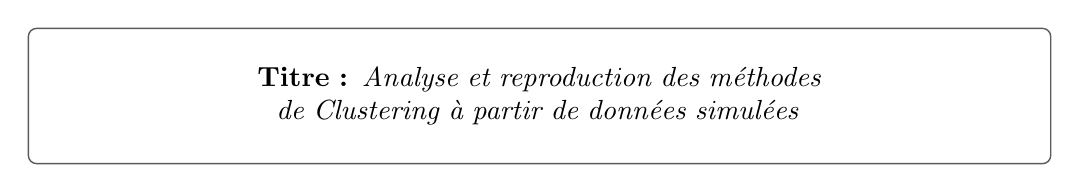
\begin{tikzpicture}
    \node[
      draw=cnamgray,
      line width=0.5pt,
      rounded corners=3pt,
      inner sep=14pt,
      text width=12cm,
      align=center,
      fill=white
    ]{%
      \textbf{Titre :} \textit{Analyse et reproduction des m\'{e}thodes de Clustering
      \`{a} partir de donn\'{e}es simul\'{e}es}%
    };
  \end{tikzpicture}
\end{center}

\vfill

\begin{center}
  \textcolor{rulegray}{\rule{10cm}{0.4pt}}\\[0.4cm]
  {\small\color{cnamgray} Ann\'{e}e universitaire 2025-2026}
\end{center}

\end{titlepage}

% ── PAGE TABLE DES MATIÈRES ────────────────────────────────── 
\newpage
\thispagestyle{empty}
\renewcommand{\contentsname}{\color{sectionblue}Table des mati\`{e}res}
{
  \hypersetup{linkcolor=sectionblue}
  \tableofcontents
}
\newpage

% ── CORPS DU DOCUMENT ──────────────────────────────────────── 
\setcounter{page}{1}
\pagestyle{fancy}

\section{L'article}\label{larticle}

Ce fichier \textbf{Quarto} utilise cet article
\textcite{clusterAnalysis}, l'objectif est de reproduire les résultats
obtenus sur le sujet du clustering. Dans cette étude, on explore les
méthodes de clustering en se basant sur des données simulées, en ayant
pour objectif de reconstituer le clustering avec des méthodes
statistiques.

\section{Importation des packages
utilisés}\label{importation-des-packages-utilisuxe9s}

\begin{Shaded}
\begin{Highlighting}[]
\FunctionTok{library}\NormalTok{(mvtnorm)}
\FunctionTok{library}\NormalTok{(MASS)}
\FunctionTok{library}\NormalTok{(dplyr)}
\FunctionTok{library}\NormalTok{(ggplot2)}
\FunctionTok{library}\NormalTok{(plot3D)}
\FunctionTok{library}\NormalTok{(gplots)}
\FunctionTok{library}\NormalTok{(tidyverse)}
\FunctionTok{library}\NormalTok{(plotly)}
\FunctionTok{library}\NormalTok{(scales)}
\FunctionTok{library}\NormalTok{(factoextra)}
\FunctionTok{library}\NormalTok{(NbClust)}
\FunctionTok{library}\NormalTok{(mclust)}
\FunctionTok{library}\NormalTok{(kableExtra)}
\FunctionTok{library}\NormalTok{(kStatistics)}
\FunctionTok{library}\NormalTok{(gridExtra)}
\end{Highlighting}
\end{Shaded}

\section{Création d'une simulation de
données}\label{cruxe9ation-dune-simulation-de-donnuxe9es}

La génération des données simulées va permettre de tester les méthodes
de clustering sur des données dont on connaît la répartition, sur
lesquels on a nous même défini les groupes. On pourra ainsi comparer les
groupes théoriques aux groupes trouvés avec les différentes fonctions.

\subsection{Génération des
données}\label{guxe9nuxe9ration-des-donnuxe9es}

Pour simuler les données, on définit une graine (seed) pour la
reproductibilité.

On détermine le nombre d'individus dans chaque groupe. On doit avoir la
répartition suivante :

\begin{itemize}
\tightlist
\item
  \textbf{Groupe 1} : 30\%
\item
  \textbf{Groupe 2} : 40\%
\item
  \textbf{Groupe 3} : 30\%
\end{itemize}

Ensuite, on fixe les coordonnées des moyennes de chaque groupe, ce sont
en fait les points moyens théoriques pour chaque groupe. Pour créer
cela, on insère les coordonnées dans une matrice (2,3)

\begin{itemize}
\tightlist
\item
  \textbf{Groupe 1} : (0,0)
\item
  \textbf{Groupe 2} : (3,5)
\item
  \textbf{Groupe 3} : (0,6)
\end{itemize}

Une fois les centres des groupes définis, il faut déterminer comment les
individus vont s'éparpiller autour de ces centres. C'est le rôle des
matrices de covariance.

\begin{itemize}
\tightlist
\item
  \textbf{\texttt{Sigma.sph\ =\ diag(c(1,\ 1))}} : Cette ligne crée une
  matrice de dispersion en forme circulaire. Concrètement, les points
  s'écarteront de la même manière dans toutes les directions.
\item
  \textbf{\texttt{Sigma.ell\ =\ matrix(...)}} : Cette ligne crée une
  matrice de dispersion en forme elliptique. Les valeurs choisies font
  que le nuage de points sera étiré.
\end{itemize}

On génère aléatoirement le cluster théoriques de 600 individus en
fonction des spécificités de la répartition des groupes, c'est à dire
que sur nos 600 individus, l'objectif de la fonction sample() est de
générer 30\% de 1 (Groupe 1), 40\% de 2 (Groupe 2), 30\% de 3 (Groupe
3).

La dernière étape place les 600 individus sur le graphique, fonction de
leur groupe :

\begin{itemize}
\tightlist
\item
  \textbf{Pour chaque individu (de 1 à 600)}, on regarde à quel groupe
  il appartient (\texttt{cl{[}i{]}}).
\item
  On utilise la fonction \texttt{rmvnorm()} qui génère des points
  aléatoires selon une Loi Normale avec une condition \texttt{ifelse} :

  \begin{itemize}
  \tightlist
  \item
    \textbf{S'il est dans le groupe 3} : on lui donne les coordonnées du
    centre du groupe 3 et on lui applique la dispersion en forme
    d'ellipse.
  \item
    \textbf{Sinon (s'il est dans le groupe 1 ou 2)} : on lui donne les
    coordonnées de son groupe et on lui applique la dispersion en forme
    circulaire.
  \end{itemize}
\end{itemize}

\subsection{Visualisation des données - Avec
MASS}\label{visualisation-des-donnuxe9es---avec-mass}

Voici la visualisation des données simulées. On distingue correctement
les 3 groupes avec une forme elliptique et deux formes circulaires. Le
package \emph{MASS} met à disposition la fonction \texttt{eqscplot()}
pour afficher le nuage de dispersion.

\pandocbounded{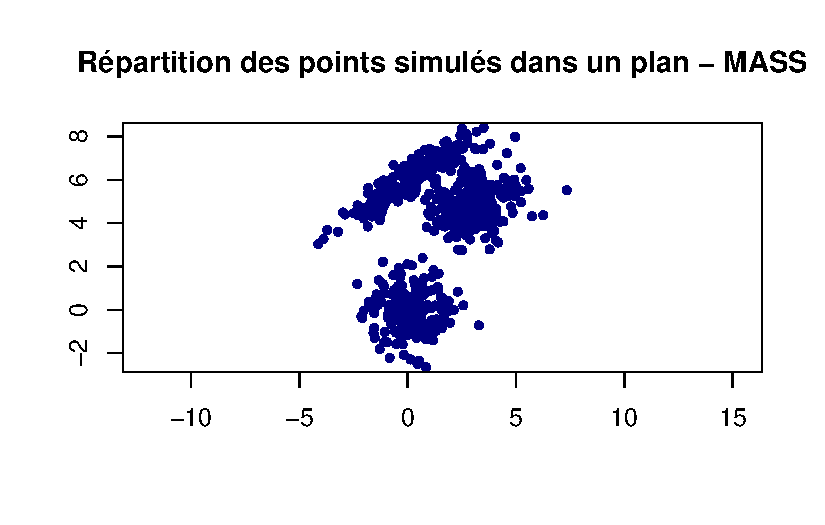
\includegraphics[keepaspectratio]{cluster_analysis_files/figure-pdf/unnamed-chunk-3-1.pdf}}

\subsection{Visualisation des données - Avec
ggplot2}\label{visualisation-des-donnuxe9es---avec-ggplot2}

On peut aussi représenter les données en utilisant le package
\emph{ggplot2} et la méthode \texttt{geom\_point()}

\pandocbounded{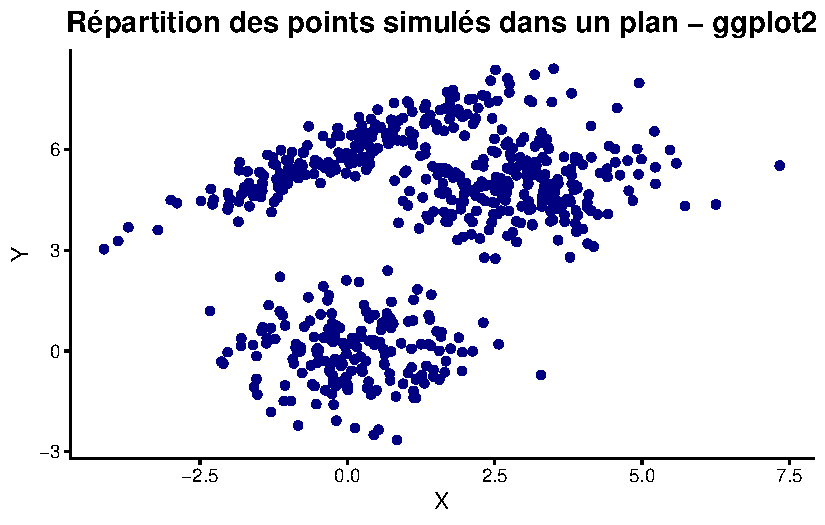
\includegraphics[keepaspectratio]{cluster_analysis_files/figure-pdf/unnamed-chunk-4-1.pdf}}

\subsection{Visualisation en 3D de l'histogramme de la loi normale
bivariée}\label{visualisation-en-3d-de-lhistogramme-de-la-loi-normale-bivariuxe9e}

On peut représenter la loi normale bivariée des données à partir d'un
plan en 3 dimensions. On retrouve bien nos 3 groupes.Les barres qui sont
rouges sont les intervalles de données plus fréquents sont mis en rouge,
ceux qui sont peu représentés sont plus en bleu. On est dans une loi
normale bivariée, de paramètre (Espérance, Matrice variance-covariance).

\pandocbounded{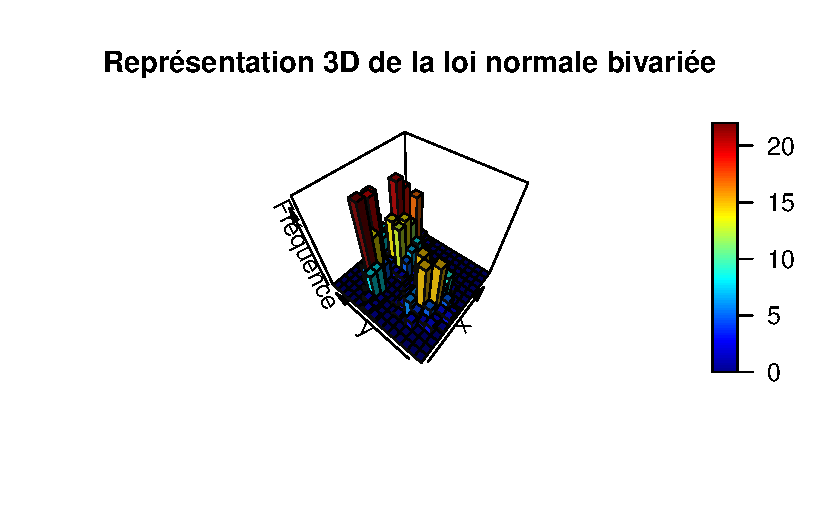
\includegraphics[keepaspectratio]{cluster_analysis_files/figure-pdf/unnamed-chunk-5-1.pdf}}

\subsection{Répartition des individus
simulés}\label{ruxe9partition-des-individus-simuluxe9s}

Le tableau ci-dessous représente les effectifs par groupe. Ils sont bien
réparti comme nous l'avons configuré. Le groupe 1 est proche de 30\%, le
groupe 2 est proche de 40\% et le groupe 3 est aussi proche de 30\%.
L'aléatoire et la seed configurés font que c'est pas parfaitement égal à
notre paramétrage.

\begin{longtable*}[t]{>{}l|ccc}
\toprule
\cellcolor[HTML]{6556E8}{\textcolor{white}{\textbf{}}} & \cellcolor[HTML]{6556E8}{\textcolor{white}{\textbf{Groupe 1}}} & \cellcolor[HTML]{6556E8}{\textcolor{white}{\textbf{Groupe 2}}} & \cellcolor[HTML]{6556E8}{\textcolor{white}{\textbf{Groupe 3}}}\\
\midrule
\textbf{Effectif} & 177 (29.5\%) & 237 (39.5\%) & 186 (31\%)\\
\bottomrule
\end{longtable*}

\subsection{Visualisation des données en fonction de leur
groupe}\label{visualisation-des-donnuxe9es-en-fonction-de-leur-groupe}

On peut représenter visuellement les groupes théoriques des données
simulées en attribuant une couleur en fonction de leur groupe.
Désormais, on distingue plus facilement les 3 groupes, notamment la
forme ellipsoidale.

\pandocbounded{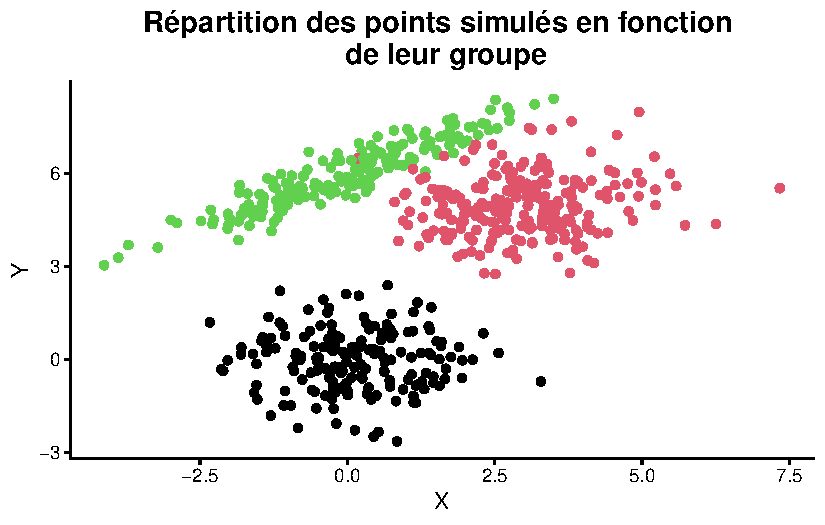
\includegraphics[keepaspectratio]{cluster_analysis_files/figure-pdf/unnamed-chunk-7-1.pdf}}

\section{Création des variables
discrètes}\label{cruxe9ation-des-variables-discruxe8tes}

\subsection{Génération des données
discrètes}\label{guxe9nuxe9ration-des-donnuxe9es-discruxe8tes}

Cette partie recréer les quatre variables discrètes (trois binaires et
une ternaire) qui accompagnent les variables continues dans le jeu de
données simulé de l'article.

Voici le détail de la construction de chaque variable pour refléter la
structure des groupes (où le groupe 1 correspond au groupe Noir, le
groupe 2 au Rouge et le groupe 3 au Vert) :

\begin{itemize}
\item
  Variable c1 : Elle est simulée avec une probabilité uniforme de 0.5
  d'obtenir un succès (valeur 2) ou un échec (valeur 1), indépendamment
  du groupe d'appartenance de l'observation.
\item
  Variable c2 : Il s'agit d'une variable binaire conçue pour avoir une
  probabilité de succès asymétrique. Le succès est beaucoup plus
  probable (0.9) pour les groupes 2 et 3 que pour le groupe 1 (0.1).
\item
  Variable c3 : C'est la variable ternaire (modalités 1, 2 et 3) de
  l'étude. Sa distribution est paramétrée pour qu'une observation ait
  une plus forte probabilité d'obtenir un 1 si elle est dans le groupe
  noir, un 2 dans le groupe rouge et un 3 dans le groupe vert.
\item
  Variable c4 : C'est une variable binaire dont la probabilité de succès
  a été configurée pour être nettement supérieure dans le groupe rouge
  (probabilité de 0.8).
\end{itemize}

{\def\LTcaptype{none} % do not increment counter
\begin{longtable}[]{@{}rrrrrr@{}}
\toprule\noalign{}
& & c1 & c2 & c3 & c4 \\
\midrule\noalign{}
\endhead
\bottomrule\noalign{}
\endlastfoot
1.6137555 & 4.6784541 & 1 & 2 & 2 & 2 \\
0.3135524 & -0.3026124 & 2 & 1 & 2 & 1 \\
3.1383011 & 3.7670414 & 2 & 2 & 2 & 1 \\
-1.5400580 & -0.1531943 & 1 & 1 & 1 & 1 \\
2.5165331 & 4.8541686 & 1 & 2 & 2 & 1 \\
1.9779610 & 4.4491698 & 1 & 2 & 2 & 2 \\
\end{longtable}
}

\subsection{Visualisation de la fréquence des
modalités}\label{visualisation-de-la-fruxe9quence-des-modalituxe9s}

Nous représentons les variables discrètes avec le graphique à barres
suivant, pour distinguer visuellement la proportion des modalités des
variables discrètes par groupe.

\pandocbounded{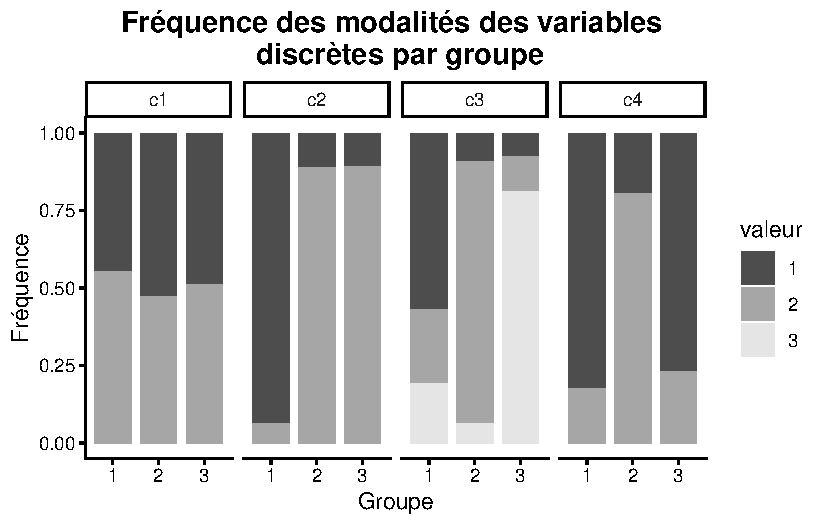
\includegraphics[keepaspectratio]{cluster_analysis_files/figure-pdf/unnamed-chunk-9-1.pdf}}

\section{Le clustering}\label{le-clustering}

\subsection{Application de la fonction
k-means}\label{application-de-la-fonction-k-means}

Nous aurions pu explorer toutes les possiblités pour 2 clusters une par
une à la main, mais c'est impossible vu le nombre de possibilités pour
600 observations. Il faudrait effectuer la démarche le nombre de fois
ci-dessous :

\begin{verbatim}
[1] 2.074758e+180
\end{verbatim}

\subsection{Méthode du coude}\label{muxe9thode-du-coude}

La méthode du coude sert définir visuellement le nombre optimal de
clusters afin de conserver le plus d'information possible. Nous devons
nous arrêter au moment où l'inertie ne chute plus de manière
significative.

Dans le graphique ci-dessous, le coude commence à se former à partir du
cluster \(k = 3\). Nous conservons donc que 3 clusters.

\pandocbounded{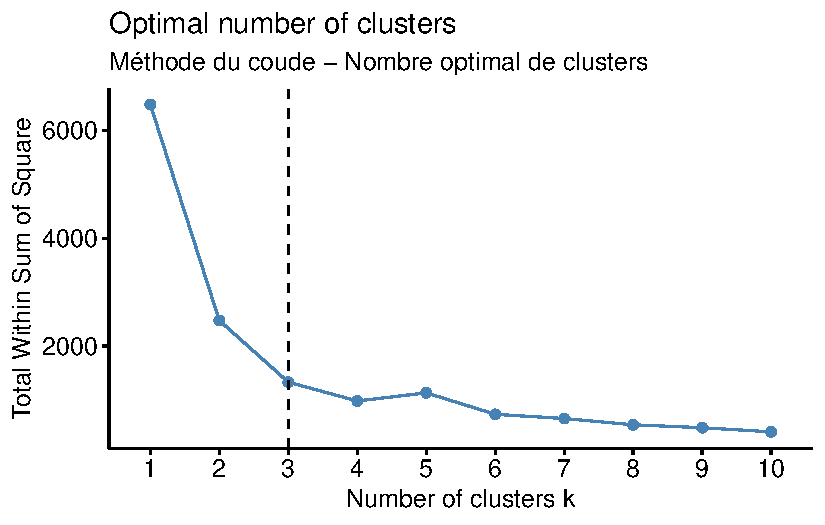
\includegraphics[keepaspectratio]{cluster_analysis_files/figure-pdf/unnamed-chunk-11-1.pdf}}

La méthode du coude est performante pour trouver le nombre de cluster
optimal mais reste très dépendante de notre interprétation.

Dans la méthode ci-dessous, la méthode ``Gap statistic'', le nombre
optimal de clusters \(k\) est celui qui donne le Gap le plus grand.
C'est une méthode plus mathématique et souvent plus robuste que la
méthode du coude visuelle.

Elle compare la dispersion intra-cluster observée dans les données à
l'espérance mathématique de cette dispersion générée sous une
distribution uniforme de référence (hypothèse nulle d'absence de
clusters). Le \(k\) optimal est la valeur qui maximise cet écart.

Avec cette méthode, on détecte automatiquement que le nombre de clusters
optimal est \(k = 3\).

\pandocbounded{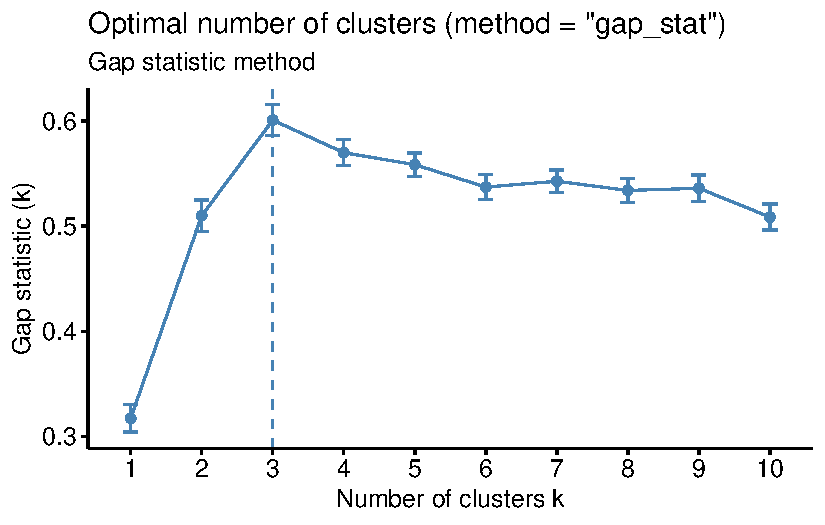
\includegraphics[keepaspectratio]{cluster_analysis_files/figure-pdf/unnamed-chunk-12-1.pdf}}

\section{Méthode des kmeans - algorithme
d'Hartigan-Wong}\label{muxe9thode-des-kmeans---algorithme-dhartigan-wong}

\subsection{L'algorithme d'Hartigan}\label{lalgorithme-dhartigan}

Description de l'algorithme d'Hartigan-Wong pour la méthode des kmeans.

\[\begin{array}{l}
\textbf{Algorithme de Hartigan-Wong (K-Means)} \\
\hline
1.\ \textbf{Initialisation : } \text{Distribuer chaque point dans un cluster au hasard.} \\
2.\ \textbf{Calcul des centres : } \text{Calculer le centre moyen de chaque groupe formé.} \\
3.\ \textbf{Boucle principale : } \text{Pour chaque point du jeu de données :} \\
\quad 4.\ \textbf{Test de transfert : } \text{Calculer si déplacer le point vers un autre groupe} \\
\quad \quad \text{rend l'ensemble des clusters plus compact.} \\
\quad 5.\ \textbf{Décision : } \text{Si le transfert améliore la qualité globale :} \\
\quad \quad 6.\ \textbf{Action : } \text{Déplacer le point dans le nouveau groupe immédiatement.} \\
\quad \quad 7.\ \textbf{Mise à jour : } \text{Recalculer aussitôt le centre du groupe qui a perdu} \\
\quad \quad \quad \text{le point et celui du groupe qui l'a gagné.} \\
8.\ \textbf{Convergence : } \text{Recommencer l'étape 3 tant que des points bougent encore.} \\
\hline
\end{array}\]

Nous avons calculé les clusters avec cette méthode en définissant le
nombre de cluster \(k = 3\). Dans ce résultat, nous avons donc
l'appartenance de chaque point à un cluster. Ensuite, on reprend le
nuage de dispersion des points simulés et on leur applique les couleurs
des clusters calculés. On compare les deux graphiques pour avoir le
graphique parfait (simulé) et le graphique avec les clusters calculés.

On peut voir que la partie du haut au niveau du croisement entre les
clusters 2 et 3, la méthode des kmeans avec l'algorithme d'Hartigan-Wong
arrive mal à définir l'appartenance au cluster puisqu'il fait des
erreurs.

\pandocbounded{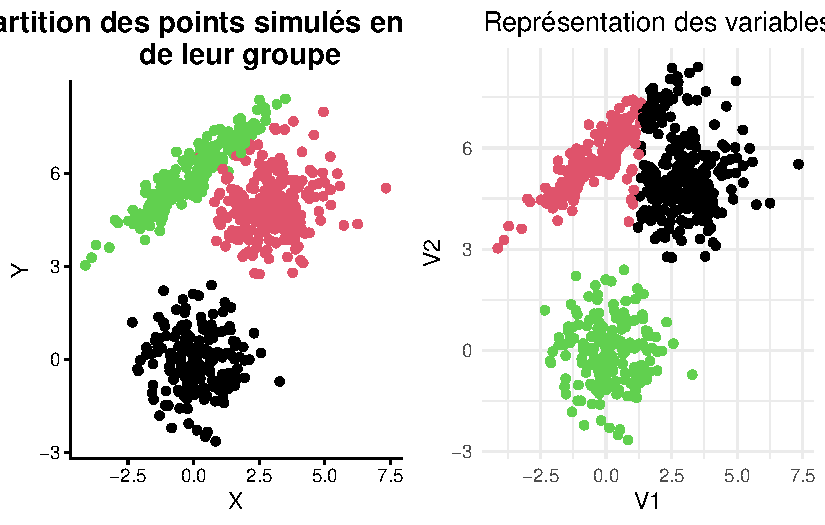
\includegraphics[keepaspectratio]{cluster_analysis_files/figure-pdf/unnamed-chunk-13-1.pdf}}

\begin{Shaded}
\begin{Highlighting}[]
\NormalTok{cl}
\end{Highlighting}
\end{Shaded}

\begin{verbatim}
  [1] 2 1 2 1 2 2 3 2 2 3 1 3 1 2 3 3 2 2 2 2 3 3 1 2 1 2 2 2 2 1 1 2 1 1 3 2 1
 [38] 1 2 1 2 3 2 1 2 3 1 2 1 3 3 1 2 3 1 1 2 3 2 2 1 1 3 3 3 2 3 2 1 1 3 2 2 3
 [75] 1 3 2 1 2 2 2 2 1 1 2 3 3 1 2 1 3 3 1 3 1 1 2 2 2 3 2 1 2 3 2 2 3 2 1 3 2
[112] 2 2 3 1 1 3 2 2 3 1 2 2 1 2 3 3 2 1 2 3 2 3 1 2 2 2 2 1 3 2 3 1 2 2 3 1 1
[149] 3 3 3 2 3 1 3 1 3 2 3 3 3 3 2 3 2 3 2 1 2 3 3 1 1 1 1 2 1 2 1 2 3 2 1 2 2
[186] 2 1 3 2 2 3 1 2 2 2 2 3 1 3 3 2 3 2 1 3 1 2 2 2 2 2 1 1 3 2 3 3 3 3 2 3 3
[223] 2 3 3 3 3 2 2 2 2 1 1 2 2 3 3 3 3 2 2 2 2 3 3 2 1 3 1 3 2 3 3 3 3 3 2 2 1
[260] 2 3 1 1 2 3 2 1 1 1 2 1 2 2 1 1 2 3 1 3 1 2 1 3 3 2 2 2 2 3 2 2 3 3 2 1 1
[297] 3 2 3 1 1 2 3 1 1 1 1 3 2 1 2 2 3 2 1 1 3 2 2 2 2 3 1 3 1 2 2 3 2 2 2 1 1
[334] 3 1 1 2 2 2 2 2 2 3 1 3 2 3 2 3 3 2 3 3 2 2 1 2 1 3 3 1 1 1 1 1 2 1 2 3 3
[371] 2 3 1 2 2 3 2 2 2 1 2 1 1 3 2 1 1 3 3 3 3 2 2 2 1 2 1 2 2 3 2 3 1 1 3 2 3
[408] 2 2 3 1 1 1 1 2 3 1 3 3 2 1 3 1 2 1 3 2 3 1 1 2 1 2 3 3 3 1 2 2 2 2 3 2 2
[445] 3 2 3 2 3 2 2 3 2 2 1 1 1 3 2 2 1 1 1 1 1 1 3 1 2 2 1 3 2 1 3 2 2 3 1 1 3
[482] 3 2 3 3 3 2 2 3 3 1 2 2 3 2 1 1 3 1 3 1 2 3 1 2 3 2 2 2 3 1 2 3 1 3 2 2 1
[519] 2 2 3 2 1 1 1 3 2 1 1 1 2 2 2 2 1 1 3 2 2 1 3 2 1 3 3 1 3 2 1 3 2 3 3 2 3
[556] 1 2 3 2 2 2 2 2 1 1 1 3 2 1 3 3 3 1 2 1 3 3 3 3 1 1 1 1 2 1 2 3 2 1 3 2 3
[593] 2 3 1 1 1 1 2 2
\end{verbatim}

\begin{Shaded}
\begin{Highlighting}[]
\NormalTok{cluster3}\SpecialCharTok{$}\NormalTok{cluster}
\end{Highlighting}
\end{Shaded}

\begin{verbatim}
  [1] 2 3 2 3 2 2 1 2 2 1 3 1 3 2 1 1 2 2 2 2 1 1 3 2 3 2 2 2 2 3 3 1 3 3 2 2 3
 [38] 3 2 3 2 1 2 3 2 1 3 2 3 2 1 3 2 2 3 3 2 1 2 2 3 3 1 1 1 1 1 2 3 3 1 2 2 1
 [75] 3 1 1 3 1 2 2 2 3 3 2 1 1 3 2 3 1 1 3 1 3 3 2 2 2 1 2 3 2 1 2 2 2 2 3 1 2
[112] 2 2 1 3 3 1 2 2 1 3 2 2 3 2 1 1 2 3 2 1 2 1 3 2 2 2 2 3 1 2 2 3 2 2 1 3 3
[149] 1 1 1 2 1 3 1 3 1 2 1 1 1 1 2 1 2 1 2 3 2 1 1 3 3 3 3 2 3 1 3 2 1 2 3 2 2
[186] 2 3 1 2 2 1 3 2 2 2 2 1 3 1 2 2 2 2 3 1 3 2 2 2 2 2 3 3 1 2 2 2 1 2 2 2 1
[223] 2 2 2 1 1 2 2 2 2 3 3 2 2 1 1 1 1 2 2 2 2 1 1 2 3 1 3 1 2 1 1 1 2 2 2 2 3
[260] 2 1 3 3 2 2 1 3 3 3 2 3 2 2 3 3 2 1 3 1 3 2 3 1 1 2 2 2 2 1 2 2 1 1 2 3 3
[297] 1 2 2 3 3 2 1 3 3 3 3 1 2 3 2 2 2 2 3 3 1 2 2 2 2 1 3 1 3 2 2 1 2 2 1 3 3
[334] 1 3 3 2 2 2 2 2 2 1 3 2 2 1 2 1 1 2 1 1 2 2 3 2 3 2 1 3 3 3 3 3 2 3 2 1 1
[371] 2 1 3 2 2 1 2 2 2 3 2 3 3 1 2 3 3 2 1 1 1 2 2 2 3 2 3 2 2 2 2 1 3 3 1 2 1
[408] 2 2 1 3 3 3 3 2 1 3 1 1 2 3 1 3 2 3 1 2 1 3 3 2 3 2 1 1 1 3 2 2 2 2 1 2 2
[445] 1 2 1 2 2 2 2 2 2 2 3 3 3 2 1 2 3 3 3 3 3 3 1 3 2 2 3 1 2 3 2 2 2 2 3 3 2
[482] 1 2 1 2 2 2 2 1 1 3 2 2 1 2 3 3 1 3 1 3 2 1 3 2 1 2 2 1 2 3 2 1 3 1 2 2 3
[519] 2 2 1 2 3 3 3 1 2 3 3 3 2 2 2 2 3 3 1 2 2 3 1 2 3 1 1 3 1 2 3 1 2 1 1 2 1
[556] 3 2 1 2 2 2 2 2 3 3 3 1 2 3 1 1 1 3 2 3 1 1 1 1 3 3 3 3 1 3 2 1 2 3 1 2 2
[593] 2 2 3 3 3 3 2 2
\end{verbatim}

\begin{Shaded}
\begin{Highlighting}[]
\FunctionTok{table}\NormalTok{(}\FunctionTok{tibble}\NormalTok{(cl, cluster3}\SpecialCharTok{$}\NormalTok{cluster))}
\end{Highlighting}
\end{Shaded}

\begin{verbatim}
   cluster3$cluster
cl    1   2   3
  1   0   0 177
  2  10 227   0
  3 153  33   0
\end{verbatim}

\begin{Shaded}
\begin{Highlighting}[]
\FunctionTok{library}\NormalTok{(clue)}
\NormalTok{solve\_correspondance }\OtherTok{=} \FunctionTok{solve\_LSAP}\NormalTok{(}\FunctionTok{table}\NormalTok{(}\FunctionTok{tibble}\NormalTok{(cl, cluster3}\SpecialCharTok{$}\NormalTok{cluster)), }\AttributeTok{maximum =} \ConstantTok{TRUE}\NormalTok{)}

\NormalTok{conf\_matrice }\OtherTok{=} \FunctionTok{table}\NormalTok{(}\FunctionTok{tibble}\NormalTok{(cl, cluster3}\SpecialCharTok{$}\NormalTok{cluster))[, solve\_correspondance]}

\DecValTok{1}\SpecialCharTok{{-}}\FunctionTok{sum}\NormalTok{(}\FunctionTok{diag}\NormalTok{(conf\_matrice))}\SpecialCharTok{/}\DecValTok{600} \CommentTok{\# le taux de points mal placés}
\end{Highlighting}
\end{Shaded}

\begin{verbatim}
[1] 0.07166667
\end{verbatim}

L'article aurait dû utiliser l'indice de Rand pour évaluer la
concordance entre les données simulées et la répartition trouvée par
kmeans(). Explicatoin du fonctionnement du Rand : L'indice de Rand est
une mesure de similarité entre deux partitions d'un ensemble. Il est
principalement utilisé en catégorisation automatique. Son principe est
de mesurer la consistance (le taux d'accord) entre deux partitions.

Prenons un exemple pour illustrer la méthode, supposons une classe qui a
9 élèves, on veut comparer les deux partitions suivante : - partition 1
: \{A,B\}, \{C,D,E,F,G\}, \{H,I\} - partition 2 : \{A\}, \{B\},
\{C,D,E\}, \{F,G\}, \{H,I\}

L'indice va compter le nombre de paires parmi les 36 qui sont soit dans
un même groupe, soit dans deux groupes différents dans la partition 1 et
la partition 2.

Dans cet exemple, on trouve 80,6\% de concordance.

\begin{Shaded}
\begin{Highlighting}[]
\FunctionTok{library}\NormalTok{(fossil)}
\end{Highlighting}
\end{Shaded}

\begin{verbatim}
Loading required package: sp
\end{verbatim}

\begin{verbatim}
Loading required package: maps
\end{verbatim}

\begin{verbatim}

Attaching package: 'maps'
\end{verbatim}

\begin{verbatim}
The following object is masked from 'package:mclust':

    map
\end{verbatim}

\begin{verbatim}
The following object is masked from 'package:purrr':

    map
\end{verbatim}

\begin{verbatim}
Loading required package: shapefiles
\end{verbatim}

\begin{verbatim}
Loading required package: foreign
\end{verbatim}

\begin{verbatim}

Attaching package: 'shapefiles'
\end{verbatim}

\begin{verbatim}
The following objects are masked from 'package:foreign':

    read.dbf, write.dbf
\end{verbatim}

\begin{Shaded}
\begin{Highlighting}[]
\NormalTok{g1 }\OtherTok{=} \FunctionTok{c}\NormalTok{(}\DecValTok{1}\NormalTok{, }\DecValTok{1}\NormalTok{,}\FunctionTok{rep}\NormalTok{(}\DecValTok{2}\NormalTok{, }\DecValTok{5}\NormalTok{), }\DecValTok{3}\NormalTok{,}\DecValTok{3}\NormalTok{)}
\NormalTok{g2 }\OtherTok{=} \FunctionTok{c}\NormalTok{(}\DecValTok{1}\NormalTok{, }\DecValTok{2}\NormalTok{, }\DecValTok{3}\NormalTok{, }\DecValTok{3}\NormalTok{, }\DecValTok{3}\NormalTok{, }\DecValTok{4}\NormalTok{, }\DecValTok{4}\NormalTok{, }\DecValTok{5}\NormalTok{, }\DecValTok{5}\NormalTok{)}

\FunctionTok{rand.index}\NormalTok{(g1, g2)}
\end{Highlighting}
\end{Shaded}

\begin{verbatim}
[1] 0.8055556
\end{verbatim}

\begin{Shaded}
\begin{Highlighting}[]
\NormalTok{(}\DecValTok{7}\SpecialCharTok{+}\DecValTok{7}\SpecialCharTok{+}\DecValTok{6}\SpecialCharTok{+}\DecValTok{6}\SpecialCharTok{+}\DecValTok{6}\SpecialCharTok{+}\DecValTok{5}\SpecialCharTok{+}\DecValTok{5}\SpecialCharTok{+}\DecValTok{8}\SpecialCharTok{+}\DecValTok{8}\NormalTok{)}\SpecialCharTok{/}\DecValTok{36}\SpecialCharTok{/}\DecValTok{2}
\end{Highlighting}
\end{Shaded}

\begin{verbatim}
[1] 0.8055556
\end{verbatim}

Application de l'indice de Rand à nos données de clustering. Le kmeans()
avec k = 3 nous donne de concordance de 90,1\%.

\begin{Shaded}
\begin{Highlighting}[]
\FunctionTok{rand.index}\NormalTok{(cl, cluster3}\SpecialCharTok{$}\NormalTok{cluster)}
\end{Highlighting}
\end{Shaded}

\begin{verbatim}
[1] 0.9090707
\end{verbatim}

La classification hiérarchique :

méthode single linkage

\begin{Shaded}
\begin{Highlighting}[]
\FunctionTok{dist}\NormalTok{(vars[, }\DecValTok{1}\SpecialCharTok{:}\DecValTok{2}\NormalTok{], }\AttributeTok{diag =} \ConstantTok{TRUE}\NormalTok{, }\AttributeTok{method =} \StringTok{"euclidean"}\NormalTok{)}\OtherTok{{-}\textgreater{}}\NormalTok{ distance}
\end{Highlighting}
\end{Shaded}

\begin{Shaded}
\begin{Highlighting}[]
\FunctionTok{library}\NormalTok{(fastcluster)}
\end{Highlighting}
\end{Shaded}

\begin{verbatim}

Attaching package: 'fastcluster'
\end{verbatim}

\begin{verbatim}
The following object is masked from 'package:stats':

    hclust
\end{verbatim}

\begin{Shaded}
\begin{Highlighting}[]
\NormalTok{arbre }\OtherTok{\textless{}{-}} \FunctionTok{hclust}\NormalTok{(distance, }\AttributeTok{method =} \StringTok{"average"}\NormalTok{)}
\FunctionTok{plot}\NormalTok{(arbre, }\AttributeTok{labels =} \ConstantTok{FALSE}\NormalTok{, }\AttributeTok{main =} \StringTok{"Dendrogramme"}\NormalTok{)}
\end{Highlighting}
\end{Shaded}

\pandocbounded{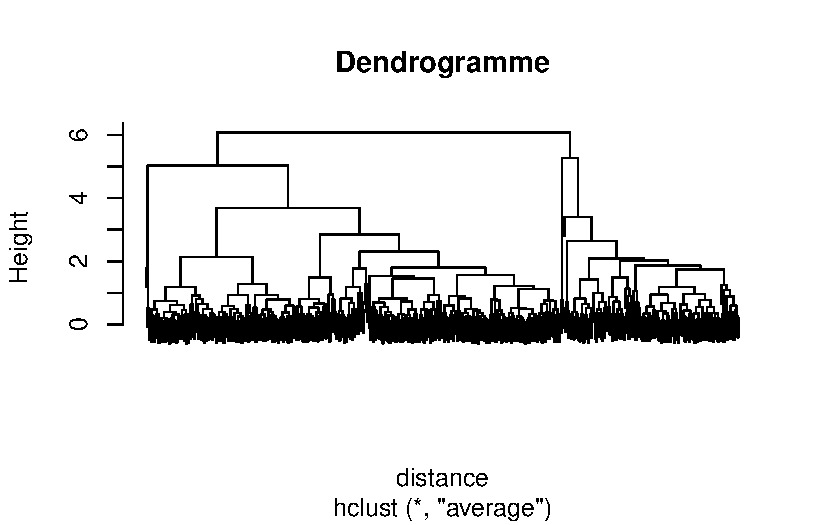
\includegraphics[keepaspectratio]{cluster_analysis_files/figure-pdf/unnamed-chunk-18-1.pdf}}

\begin{Shaded}
\begin{Highlighting}[]
\FunctionTok{library}\NormalTok{(sparcl)}
\FunctionTok{ColorDendrogram}\NormalTok{(arbre, }\AttributeTok{y =}\NormalTok{ cl, }\AttributeTok{main=}\StringTok{"Single Linkage"}\NormalTok{, }\AttributeTok{xlab =} \StringTok{""}\NormalTok{, }\AttributeTok{sub =} \StringTok{""}\NormalTok{, }\AttributeTok{cex =}\NormalTok{ .}\DecValTok{75}\NormalTok{)}
\end{Highlighting}
\end{Shaded}

\pandocbounded{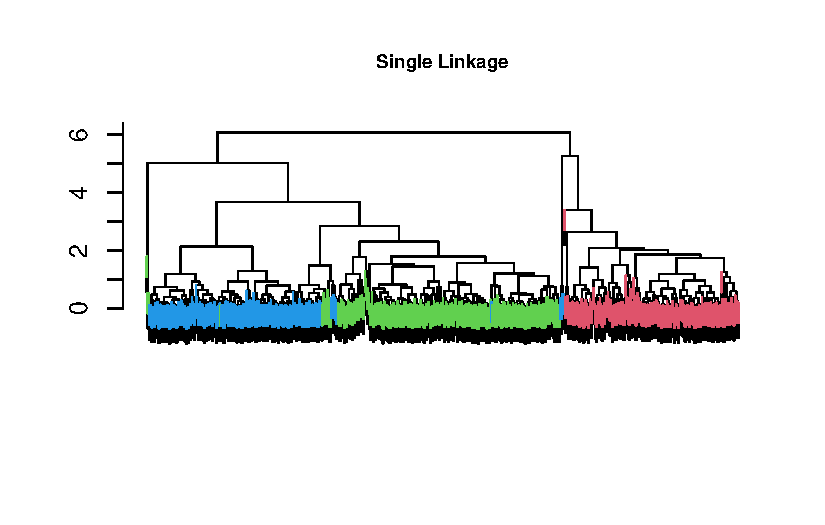
\includegraphics[keepaspectratio]{cluster_analysis_files/figure-pdf/unnamed-chunk-19-1.pdf}}

\begin{Shaded}
\begin{Highlighting}[]
\FunctionTok{rand.index}\NormalTok{(cl, }\FunctionTok{cutree}\NormalTok{(arbre, }\AttributeTok{k=}\DecValTok{3}\NormalTok{))}
\end{Highlighting}
\end{Shaded}

\begin{verbatim}
[1] 0.7559154
\end{verbatim}

\begin{Shaded}
\begin{Highlighting}[]
\NormalTok{solve\_correspondance\_arbre }\OtherTok{=} \FunctionTok{solve\_LSAP}\NormalTok{(}\FunctionTok{table}\NormalTok{(}\FunctionTok{tibble}\NormalTok{(cl, }\FunctionTok{cutree}\NormalTok{(arbre, }\AttributeTok{k=}\DecValTok{3}\NormalTok{))), }\AttributeTok{maximum =} \ConstantTok{TRUE}\NormalTok{)}

\NormalTok{conf\_matrice\_arbre }\OtherTok{=} \FunctionTok{table}\NormalTok{(}\FunctionTok{tibble}\NormalTok{(cl, }\FunctionTok{cutree}\NormalTok{(arbre, }\AttributeTok{k=}\DecValTok{3}\NormalTok{)))[, solve\_correspondance\_arbre]}
\NormalTok{conf\_matrice\_arbre}
\end{Highlighting}
\end{Shaded}

\begin{verbatim}
   cutree(arbre, k = 3)
cl    2   1   3
  1 177   0   0
  2   0 237   0
  3   0 182   4
\end{verbatim}

\subsection{Illustration avec 10
individus:}\label{illustration-avec-10-individus}

\begin{Shaded}
\begin{Highlighting}[]
\FunctionTok{cbind}\NormalTok{(X, cl) }\OtherTok{{-}\textgreater{}}\NormalTok{ data\_10}

\NormalTok{data\_10 }\SpecialCharTok{\%\textgreater{}\%} \FunctionTok{as\_tibble}\NormalTok{() }\SpecialCharTok{\%\textgreater{}\%} \FunctionTok{arrange}\NormalTok{(cl) }\SpecialCharTok{\%\textgreater{}\%} \FunctionTok{slice}\NormalTok{(}\DecValTok{1}\SpecialCharTok{:}\DecValTok{3}\NormalTok{, }\DecValTok{178}\SpecialCharTok{:}\DecValTok{181}\NormalTok{, }\DecValTok{598}\SpecialCharTok{:}\DecValTok{600}\NormalTok{)}\OtherTok{{-}\textgreater{}}\NormalTok{ data\_10}
\NormalTok{cluster\_10 }\OtherTok{=} \FunctionTok{kmeans}\NormalTok{ (data\_10, }\DecValTok{3}\NormalTok{, }\AttributeTok{nstart =} \DecValTok{50}\NormalTok{)}
\FunctionTok{dist}\NormalTok{(data\_10[,}\DecValTok{1}\SpecialCharTok{:}\DecValTok{2}\NormalTok{], }\AttributeTok{diag =} \ConstantTok{TRUE}\NormalTok{, }\AttributeTok{method =} \StringTok{"euclidean"}\NormalTok{)}\OtherTok{{-}\textgreater{}}\NormalTok{ distance\_10}
\NormalTok{arbre\_10 }\OtherTok{\textless{}{-}} \FunctionTok{hclust}\NormalTok{(distance\_10, }\AttributeTok{method =} \StringTok{"average"}\NormalTok{)}
\FunctionTok{plot}\NormalTok{(arbre\_10, }\AttributeTok{main =} \StringTok{"Dendrogramme"}\NormalTok{)}
\end{Highlighting}
\end{Shaded}

\pandocbounded{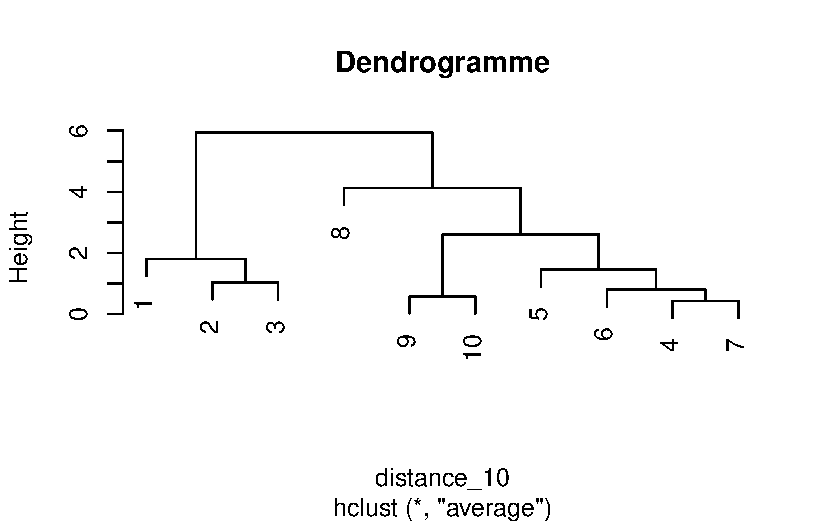
\includegraphics[keepaspectratio]{cluster_analysis_files/figure-pdf/unnamed-chunk-21-1.pdf}}

\begin{Shaded}
\begin{Highlighting}[]
\FunctionTok{ColorDendrogram}\NormalTok{(arbre\_10, }\AttributeTok{y =}\NormalTok{ data\_10}\SpecialCharTok{$}\NormalTok{cl, }\AttributeTok{main=}\StringTok{"Single Linkage"}\NormalTok{, }\AttributeTok{xlab =} \StringTok{""}\NormalTok{, }\AttributeTok{sub =} \StringTok{""}\NormalTok{, }\AttributeTok{cex =}\NormalTok{ .}\DecValTok{75}\NormalTok{, }\AttributeTok{labels =} \FunctionTok{row.names}\NormalTok{(data\_10)) }\OtherTok{{-}\textgreater{}}\NormalTok{ graph\_10\_1}
\end{Highlighting}
\end{Shaded}

\pandocbounded{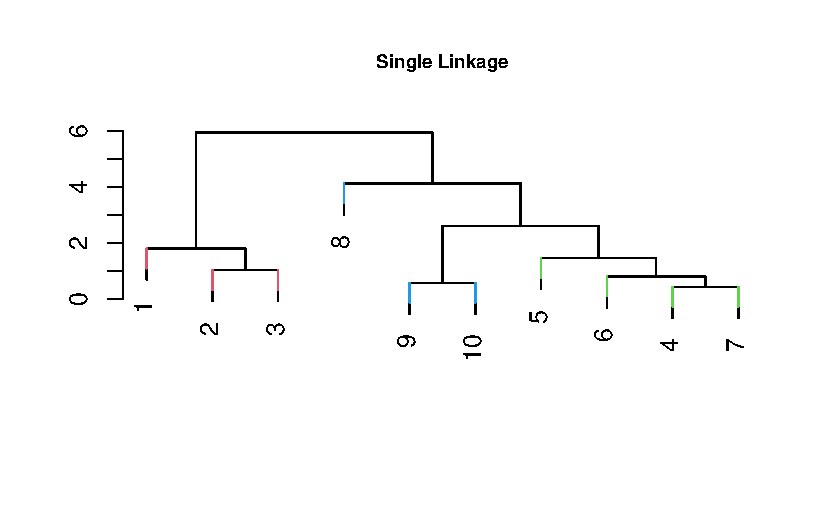
\includegraphics[keepaspectratio]{cluster_analysis_files/figure-pdf/unnamed-chunk-21-2.pdf}}

\begin{Shaded}
\begin{Highlighting}[]
\NormalTok{data\_10 }\SpecialCharTok{\%\textgreater{}\%} \FunctionTok{as.data.frame}\NormalTok{() }\SpecialCharTok{\%\textgreater{}\%} \FunctionTok{ggplot}\NormalTok{(}\FunctionTok{aes}\NormalTok{(}\AttributeTok{x =}\NormalTok{ V1, }\AttributeTok{y =}\NormalTok{ V2, }\AttributeTok{label =}\FunctionTok{row.names}\NormalTok{(data\_10)))}\SpecialCharTok{+}
  \FunctionTok{geom\_point}\NormalTok{(}\FunctionTok{aes}\NormalTok{(}\AttributeTok{color =} \FunctionTok{factor}\NormalTok{(data\_10}\SpecialCharTok{$}\NormalTok{cl)), }\AttributeTok{size =} \FloatTok{2.5}\NormalTok{)}\SpecialCharTok{+}\FunctionTok{geom\_text}\NormalTok{(}\AttributeTok{hjust =} \DecValTok{2}\NormalTok{)}\SpecialCharTok{+}
  \FunctionTok{theme\_minimal}\NormalTok{() }\OtherTok{{-}\textgreater{}}\NormalTok{ graph\_10\_2}

\FunctionTok{cbind}\NormalTok{(graph\_10\_1, graph\_10\_2)}
\end{Highlighting}
\end{Shaded}

\begin{verbatim}
     graph_10_2       
[1,] <ggplot2::ggplot>
\end{verbatim}

\begin{Shaded}
\begin{Highlighting}[]
\FunctionTok{library}\NormalTok{(dendextend)}
\end{Highlighting}
\end{Shaded}

\begin{verbatim}

---------------------
Welcome to dendextend version 1.19.1
Type citation('dendextend') for how to cite the package.

Type browseVignettes(package = 'dendextend') for the package vignette.
The github page is: https://github.com/talgalili/dendextend/

Suggestions and bug-reports can be submitted at: https://github.com/talgalili/dendextend/issues
You may ask questions at stackoverflow, use the r and dendextend tags: 
     https://stackoverflow.com/questions/tagged/dendextend

    To suppress this message use:  suppressPackageStartupMessages(library(dendextend))
---------------------
\end{verbatim}

\begin{verbatim}

Attaching package: 'dendextend'
\end{verbatim}

\begin{verbatim}
The following object is masked from 'package:stats':

    cutree
\end{verbatim}

\begin{Shaded}
\begin{Highlighting}[]
\FunctionTok{library}\NormalTok{(circlize)}
\end{Highlighting}
\end{Shaded}

\begin{verbatim}
========================================
circlize version 0.4.18
CRAN page: https://cran.r-project.org/package=circlize
Github page: https://github.com/jokergoo/circlize
Documentation: https://jokergoo.github.io/circlize_book/book/

If you use it in published research, please cite:
Gu, Z. circlize implements and enhances circular visualization
  in R. Bioinformatics 2014.

This message can be suppressed by:
  suppressPackageStartupMessages(library(circlize))
========================================
\end{verbatim}

\begin{Shaded}
\begin{Highlighting}[]
\CommentTok{\# Hierarchical clustering dendrogram}
\NormalTok{hc }\OtherTok{\textless{}{-}} \FunctionTok{as.dendrogram}\NormalTok{(arbre)}

\CommentTok{\# Circular dendrogram}
\FunctionTok{circlize\_dendrogram}\NormalTok{(hc,}
                    \AttributeTok{labels\_track\_height =} \ConstantTok{NA}\NormalTok{,}
                    \AttributeTok{dend\_track\_height =} \FloatTok{0.5}\NormalTok{,}
                    \AttributeTok{labels =} \ConstantTok{FALSE}\NormalTok{)}
\end{Highlighting}
\end{Shaded}

\pandocbounded{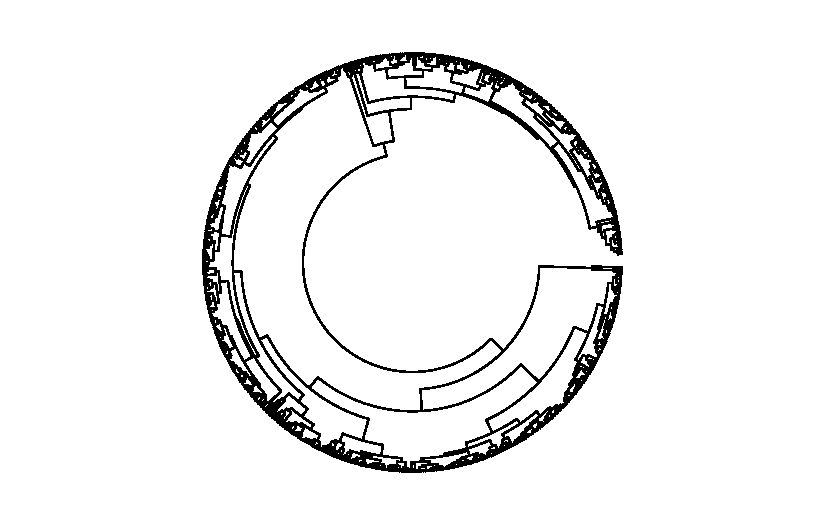
\includegraphics[keepaspectratio]{cluster_analysis_files/figure-pdf/unnamed-chunk-22-1.pdf}}

\subsubsection{kmeans - Lloyd}\label{kmeans---lloyd}

\textbf{Algo de Lloyd}

\[\begin{array}{l}
\textbf{Algorithme de Lloyd (K-Means)} \\
\hline
1.\ \textbf{Initialisation : } \text{Choisir } k \text{ points au hasard pour être les centres.} \\
2.\ \textbf{Boucle principale : } \textbf{Répéter tant qu'il y a des changements :} \\
\quad 3.\ \textbf{Assignation globale : } \text{Chaque point choisit le centre le plus} \\
\quad \quad \text{proche sans se soucier des autres points.} \\
\quad 4.\ \textbf{Attente : } \text{On attend que TOUS les points aient choisi leur groupe.} \\
\quad 5.\ \textbf{Mise à jour groupée : } \text{Une fois que tout le monde a fini de bouger,} \\
\quad \quad \text{on recalcule tous les nouveaux centres en une seule fois.} \\
6.\ \textbf{Convergence : } \text{Arrêter quand les centres ne bougent plus d'une étape à l'autre.} \\
\hline
\end{array}\]

\begin{Shaded}
\begin{Highlighting}[]
\NormalTok{cluster3\_lloyd }\OtherTok{=} \FunctionTok{kmeans}\NormalTok{ (vars [,}\DecValTok{1}\SpecialCharTok{:}\DecValTok{2}\NormalTok{], }\DecValTok{3}\NormalTok{, }\AttributeTok{nstart =} \DecValTok{50}\NormalTok{, }\AttributeTok{algorithm =} \StringTok{"Lloyd"}\NormalTok{)}
\end{Highlighting}
\end{Shaded}

\begin{verbatim}
Warning: did not converge in 10 iterations
Warning: did not converge in 10 iterations
Warning: did not converge in 10 iterations
Warning: did not converge in 10 iterations
Warning: did not converge in 10 iterations
Warning: did not converge in 10 iterations
Warning: did not converge in 10 iterations
Warning: did not converge in 10 iterations
Warning: did not converge in 10 iterations
Warning: did not converge in 10 iterations
Warning: did not converge in 10 iterations
Warning: did not converge in 10 iterations
Warning: did not converge in 10 iterations
\end{verbatim}

\begin{Shaded}
\begin{Highlighting}[]
\FunctionTok{as\_tibble}\NormalTok{(X) }\SpecialCharTok{\%\textgreater{}\%} \FunctionTok{ggplot}\NormalTok{(}\FunctionTok{aes}\NormalTok{(}\AttributeTok{x =}\NormalTok{ V1, }\AttributeTok{y=}\NormalTok{V2)) }\SpecialCharTok{+} \FunctionTok{geom\_point}\NormalTok{(}\AttributeTok{color =}\NormalTok{ cluster3\_lloyd}\SpecialCharTok{$}\NormalTok{cluster) }\SpecialCharTok{+} \FunctionTok{theme\_minimal}\NormalTok{() }\SpecialCharTok{+} \FunctionTok{ggtitle}\NormalTok{(}\StringTok{"Représentation des variables continues en fonction des groupes prédéfinis"}\NormalTok{)}
\end{Highlighting}
\end{Shaded}

\pandocbounded{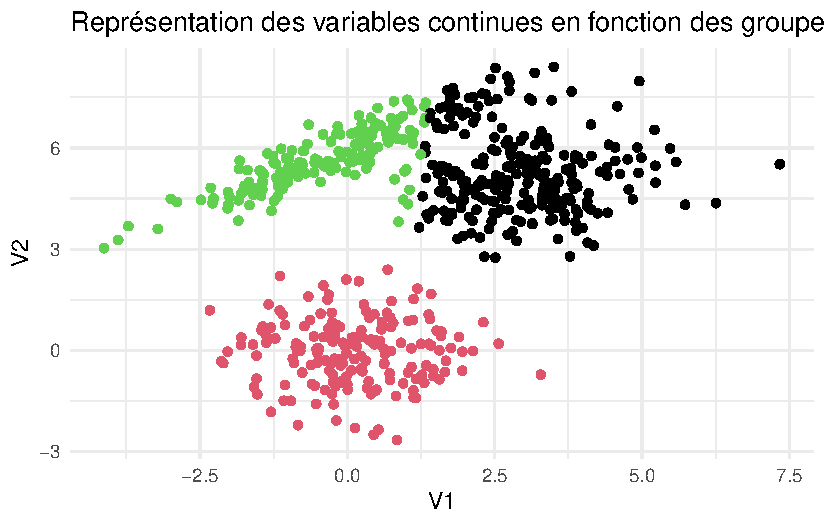
\includegraphics[keepaspectratio]{cluster_analysis_files/figure-pdf/unnamed-chunk-23-1.pdf}}

ESSAYER L4AUTRE METHODE

\subsubsection{Représentation de l'enveloppe
convexe}\label{repruxe9sentation-de-lenveloppe-convexe}

\begin{Shaded}
\begin{Highlighting}[]
\CommentTok{\# 1. Combiner vos données, la couleur d\textquotesingle{}origine (cl) et les résultats du k{-}means}
\NormalTok{df }\OtherTok{\textless{}{-}} \FunctionTok{as\_tibble}\NormalTok{(X) }\SpecialCharTok{\%\textgreater{}\%}
  \FunctionTok{mutate}\NormalTok{(}
    \AttributeTok{Couleur\_Origine =}\NormalTok{ cl,}
    \CommentTok{\# On extrait les affectations aux clusters de l\textquotesingle{}objet kmeans en facteur}
    \AttributeTok{Cluster\_Kmeans =} \FunctionTok{as.factor}\NormalTok{(cluster3\_lloyd}\SpecialCharTok{$}\NormalTok{cluster) }
\NormalTok{  )}

\CommentTok{\# 2. Calculer les points formant l\textquotesingle{}enveloppe convexe pour CHAQUE cluster k{-}means}
\CommentTok{\# La fonction chull() renvoie les indices des points qui forment la bordure convexe}
\NormalTok{hulls }\OtherTok{\textless{}{-}}\NormalTok{ df }\SpecialCharTok{\%\textgreater{}\%}
  \FunctionTok{group\_by}\NormalTok{(Cluster\_Kmeans) }\SpecialCharTok{\%\textgreater{}\%}
  \FunctionTok{slice}\NormalTok{(}\FunctionTok{chull}\NormalTok{(V1, V2))}

\CommentTok{\# 3. Créer le graphique combiné}
\FunctionTok{ggplot}\NormalTok{(df, }\FunctionTok{aes}\NormalTok{(}\AttributeTok{x =}\NormalTok{ V1, }\AttributeTok{y =}\NormalTok{ V2)) }\SpecialCharTok{+}
  \CommentTok{\# Étape A : Tracer les enveloppes convexes (polygones) des K{-}means}
  \CommentTok{\# alpha = 0.3 permet de rendre la surface transparente pour voir les points}
  \FunctionTok{geom\_polygon}\NormalTok{(}\AttributeTok{data =}\NormalTok{ hulls, }
               \FunctionTok{aes}\NormalTok{(}\AttributeTok{fill =}\NormalTok{ Cluster\_Kmeans, }\AttributeTok{group =}\NormalTok{ Cluster\_Kmeans), }
               \AttributeTok{alpha =} \FloatTok{0.3}\NormalTok{, }\AttributeTok{color =} \StringTok{"black"}\NormalTok{, }\AttributeTok{linetype =} \StringTok{"dashed"}\NormalTok{) }\SpecialCharTok{+}
  \FunctionTok{scale\_fill\_manual}\NormalTok{(}\AttributeTok{values =} \FunctionTok{c}\NormalTok{(}\StringTok{"\#FAADAD"}\NormalTok{, }\StringTok{"\#ADB4FA"}\NormalTok{, }\StringTok{"\#ADFABA"}\NormalTok{))}\SpecialCharTok{+}
               
  \CommentTok{\# Étape B : Tracer les points avec leurs couleurs d\textquotesingle{}origine (groupes prédéfinis)}
  \FunctionTok{geom\_point}\NormalTok{(}\FunctionTok{aes}\NormalTok{(}\AttributeTok{color =} \FunctionTok{factor}\NormalTok{(Couleur\_Origine))) }\SpecialCharTok{+}
  
  \CommentTok{\# Esthétique}
  \FunctionTok{theme\_minimal}\NormalTok{() }\SpecialCharTok{+}
  \FunctionTok{ggtitle}\NormalTok{(}\StringTok{"Représentation des variables continues en fonction des groupes prédéfinis}\SpecialCharTok{\textbackslash{}n}\StringTok{et enveloppes convexes des K{-}means"}\NormalTok{) }\SpecialCharTok{+}
  \FunctionTok{labs}\NormalTok{(}\AttributeTok{fill =} \StringTok{"Clusters K{-}means"}\NormalTok{, }\AttributeTok{color =} \StringTok{"Groupes initiaux"}\NormalTok{) }
\end{Highlighting}
\end{Shaded}

\pandocbounded{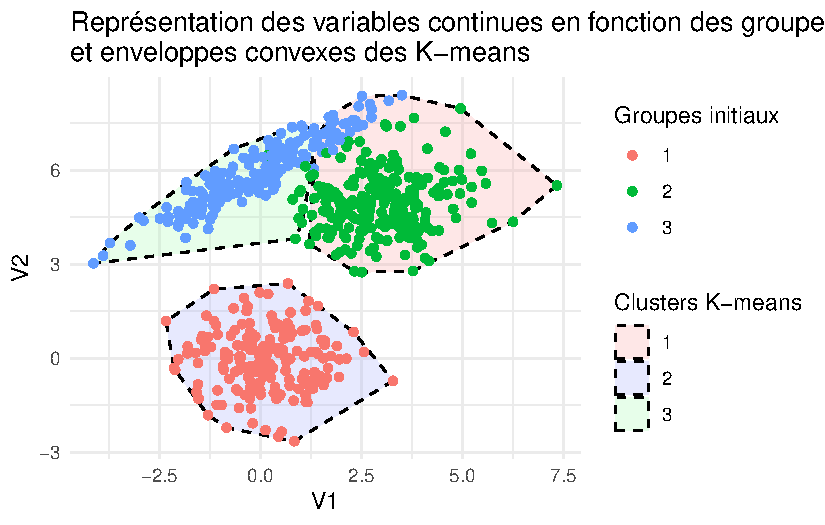
\includegraphics[keepaspectratio]{cluster_analysis_files/figure-pdf/unnamed-chunk-24-1.pdf}}

\begin{Shaded}
\begin{Highlighting}[]
\FunctionTok{fviz\_cluster}\NormalTok{(cluster3\_lloyd, }
             \AttributeTok{data =}\NormalTok{ vars[, }\DecValTok{1}\SpecialCharTok{:}\DecValTok{2}\NormalTok{], }
             \AttributeTok{ellipse.type =} \StringTok{"convex"}\NormalTok{,}
             \AttributeTok{geom =} \StringTok{"point"}\NormalTok{, }\CommentTok{\# "point" évite d\textquotesingle{}afficher le numéro de chaque ligne}
             \AttributeTok{show.clust.cent =} \ConstantTok{TRUE}\NormalTok{, }\CommentTok{\# Affiche le centre des clusters (croix)}
             \AttributeTok{main =} \StringTok{"Représentation des clusters K{-}means"}\NormalTok{)}
\end{Highlighting}
\end{Shaded}

\pandocbounded{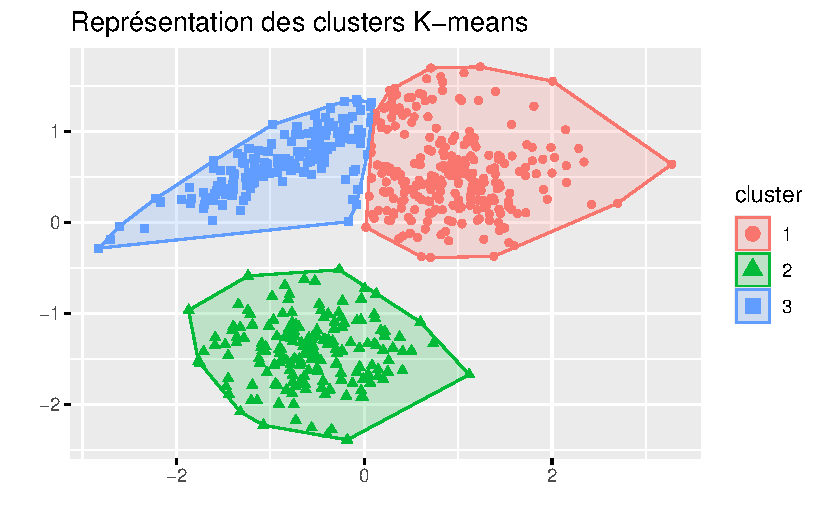
\includegraphics[keepaspectratio]{cluster_analysis_files/figure-pdf/unnamed-chunk-25-1.pdf}}

\subsection{Clustering Methods Based}\label{clustering-methods-based}

EXPLIQUER LE PRINCIPE

on est dans le cas multivariée

C'est le maximum de vraisemblance, avec le BIC le plus grand

Après on compare la simulation avec cette méthode

\begin{Shaded}
\begin{Highlighting}[]
\CommentTok{\#Fit the mbc model for a range of number of components, default 1 to 9 and all variance parameterisations on the continuous variables in the first two columns of the vars matrix}
\NormalTok{m1 }\OtherTok{=} \FunctionTok{Mclust}\NormalTok{(vars[,}\DecValTok{1}\SpecialCharTok{:}\DecValTok{2}\NormalTok{])}
\NormalTok{m1}
\end{Highlighting}
\end{Shaded}

\begin{verbatim}
'Mclust' model object: (VVE,3) 

Available components: 
 [1] "call"           "data"           "modelName"      "n"             
 [5] "d"              "G"              "BIC"            "loglik"        
 [9] "df"             "bic"            "icl"            "hypvol"        
[13] "parameters"     "z"              "classification" "uncertainty"   
\end{verbatim}

\begin{Shaded}
\begin{Highlighting}[]
\CommentTok{\#\textquotesingle{}Mclust\textquotesingle{} model object:}
\CommentTok{\#  best model: ellipsoidal, equal orientation (VVE) with 3 components}

\CommentTok{\#Look at the summary of the model}
\FunctionTok{summary}\NormalTok{(m1)}
\end{Highlighting}
\end{Shaded}

\begin{verbatim}
---------------------------------------------------- 
Gaussian finite mixture model fitted by EM algorithm 
---------------------------------------------------- 

Mclust VVE (ellipsoidal, equal orientation) model with 3 components: 

 log-likelihood   n df       BIC      ICL
      -2230.692 600 15 -4557.338 -4572.94

Clustering table:
  1   2   3 
229 177 194 
\end{verbatim}

\begin{Shaded}
\begin{Highlighting}[]
\CommentTok{\#m1$parameters}
\end{Highlighting}
\end{Shaded}

\begin{Shaded}
\begin{Highlighting}[]
\CommentTok{\#{-}{-}{-}{-}{-}{-}{-}{-}{-}{-}{-}{-}{-}{-}{-}{-}{-}{-}{-}{-}{-}{-}{-}{-}{-}{-}{-}{-}{-}{-}{-}{-}{-}{-}{-}{-}{-}{-}{-}{-}{-}{-}{-}{-}{-}{-}{-}{-}{-}{-}{-}{-}}
\CommentTok{\#  Gaussian finite mixture model fitted by EM algorithm }
\CommentTok{\#{-}{-}{-}{-}{-}{-}{-}{-}{-}{-}{-}{-}{-}{-}{-}{-}{-}{-}{-}{-}{-}{-}{-}{-}{-}{-}{-}{-}{-}{-}{-}{-}{-}{-}{-}{-}{-}{-}{-}{-}{-}{-}{-}{-}{-}{-}{-}{-}{-}{-}{-}{-}}
  
\CommentTok{\#  Mclust VVE (ellipsoidal, equal orientation) model with 3 components:}
  
\CommentTok{\#  log.likelihood   n df       BIC       ICL}
\CommentTok{\#{-}2230.702 600 15 {-}4557.359 {-}4572.325}

\CommentTok{\#Clustering table:}
\CommentTok{\#  1   2   3 }
\CommentTok{\#229 177 194 }

\CommentTok{\#Look at the BIC, classification and other plots for this model}
\FunctionTok{plot}\NormalTok{(m1)}
\end{Highlighting}
\end{Shaded}

\pandocbounded{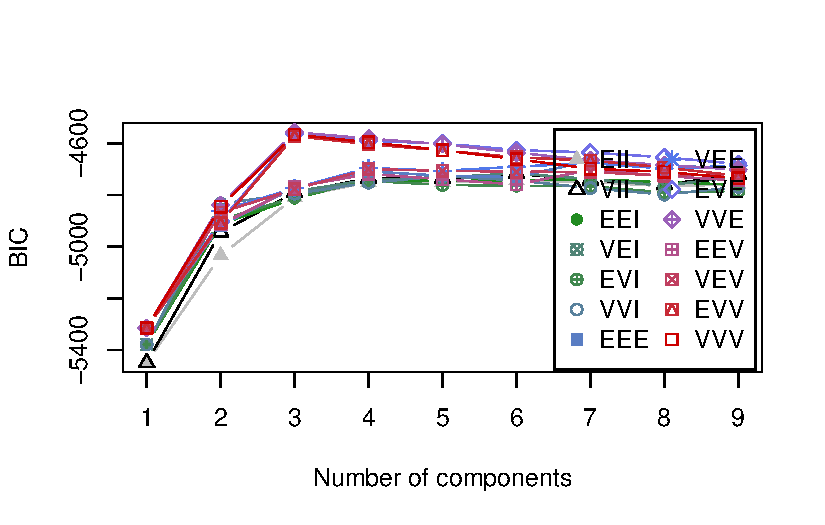
\includegraphics[keepaspectratio]{cluster_analysis_files/figure-pdf/unnamed-chunk-27-1.pdf}}

\pandocbounded{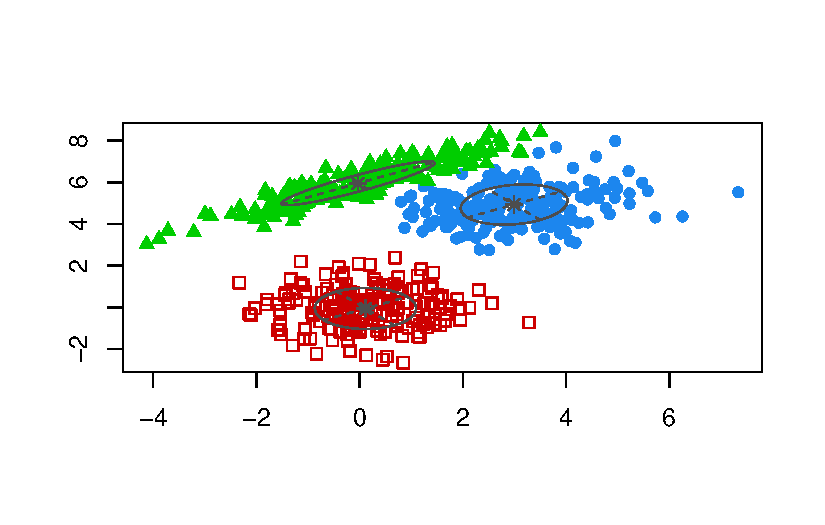
\includegraphics[keepaspectratio]{cluster_analysis_files/figure-pdf/unnamed-chunk-27-2.pdf}}

\pandocbounded{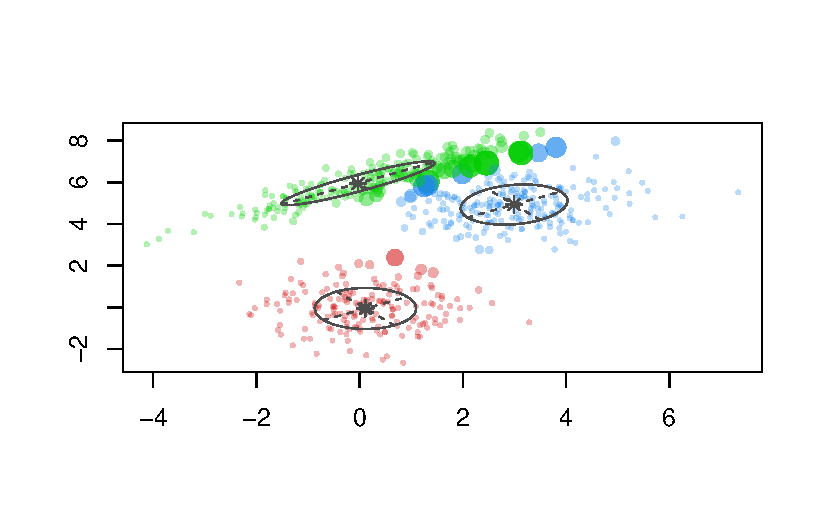
\includegraphics[keepaspectratio]{cluster_analysis_files/figure-pdf/unnamed-chunk-27-3.pdf}}

\pandocbounded{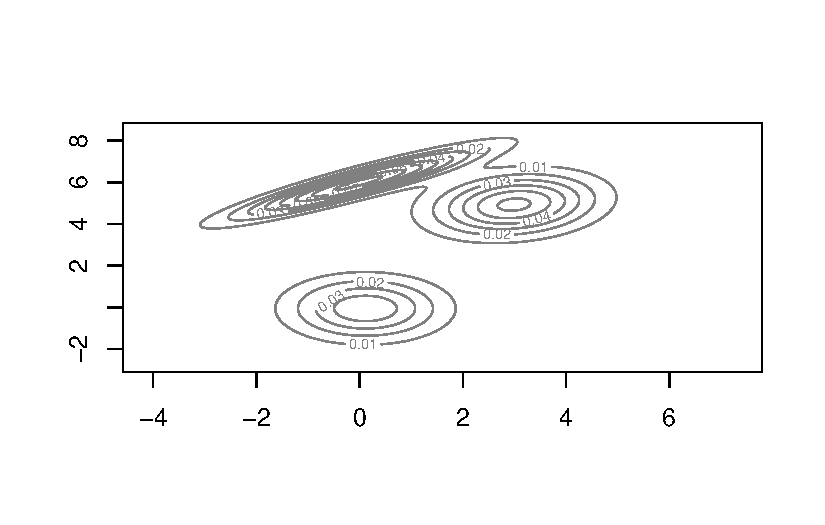
\includegraphics[keepaspectratio]{cluster_analysis_files/figure-pdf/unnamed-chunk-27-4.pdf}}

\begin{Shaded}
\begin{Highlighting}[]
\CommentTok{\# cross{-}classification table}
\CommentTok{\#table(cl, m1$class)}
\end{Highlighting}
\end{Shaded}


% ── BIBLIOGRAPHIE ──────────────────────────────────────────── 
\newpage
\printbibliography

\end{document}
